\begin{center}
	\section{Sedimentaci\'on}
\end{center}

\noindent
\justify

Se plantea que el \textit{principio funcional} del sistema de eluci\'on y filtrado de la planta de extracci\'on recaiga sobre este fen\'omeno natural.

\noindent
\justify

Los tanques de sedimentaci\'on han sido ampliamente usados como medios filtrantes en plantas purificadoras de agua debido a su capacidad de remoci\'on de residuos s\'olidos; siendo empleadas para limpiar aguas con turbidez\footnote{La turbidez define el nivel de transparencia de fluidos incoloros en contraste a la presencia de part\'iculas en suspensi\'on.} de hasta $50 [NTU]^{\cite{Voutchkov2017}}$\footnote{La Organizaci\'on Mundial de la Salud estipula que el agua de consumo humano debe presentar un nivel de turbidez inferior a $2 [NTU]^{\cite{OMSagua}}$.}. 

\noindent
\justify

Para asegurar un correcto nivel de turbidez, los sistemas de sedimentaci\'on convencionales emplean coagulantes (normalmente sales de hierro) y floculantes (pol\'imeros) en el sistema de alimentaci\'on. Cuando el fluido excede el nivel de $50 [NTU]$, se recomienda emplear sistemas de sedimentaci\'on de placas inclinadas$^{\cite{Voutchkov2017}}$ para la remoci\'on de elementos s\'olidos de bajo tama\~no de part\'icula.


\subsection{Sedimentadores convencionales}

\noindent
\justify

Son ampliamente usados para la remoci\'on de part\'iculas en fluidos con turbidez de $20 [NTU]^{\cite{Voutchkov2017}}$. Consiste de un sistema de una sola etapa estructurado de forma circular o rectangular. A la fecha, sedimentadores rectangulares se emplean sistemas de pretratamiento de aguas salinas por su bajo costo de inversi\'on y gran desempe\~no. Los par\'ametros clave para el dise\~no de estos sistemas son los siguientes:

\begin{itemize}
	\item N\'umero m\'inimo de tanques: 4
	\item Produndidad del agua: $3.0 - 4.0 [m]$.
	\item Velocidad media de flujo: $0.3 - 1.1 [m/min]$.
	\item Tiempo de detenci\'on: $2 - 4 [h]$.
	\item Relaci\'on ancho-largo: m\'inimo de 4:1.
	\item Relaci\'on profundidad-largo: m\'inimo de 1:15 
	\item Velocidad del recolector de lodos: $0.4 - 0.8 [m/min]$.
\end{itemize}

\newpage

\subsection{Sedimentador de placas inclinadas}

\noindent
\justify

Estos tanques de sedimentaci\'on, tambi\'en conocidos como \textit{clarificadores}, tienen un desempe\~no altamente superior a los convencionales, llegando a clarificar fluidos de hasta $200 [NTU]^{\cite{Voutchkov2017}}$ de turbidez. Normalmente tienen una estructura rectangular o circular y son ampliamente usados para la limpieza de agua marina. 

\begin{figure}[h!]
	\centering
	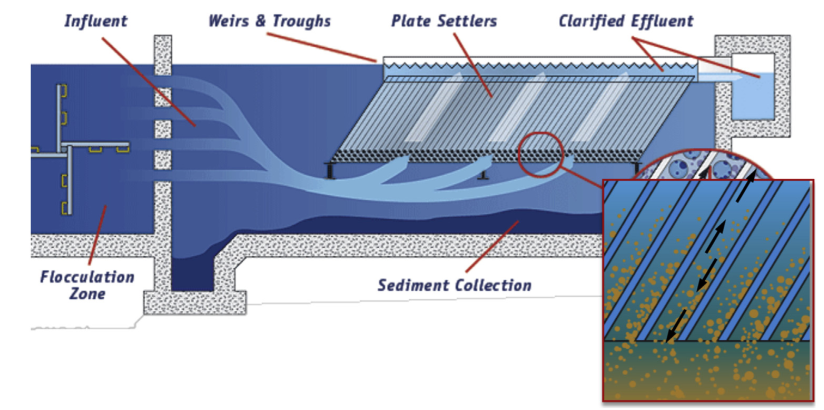
\includegraphics[width=\textwidth]{Images/lamelas_inclinadas.png}
	\caption{Esquema de un sedimentador de placas inclinadas$^{\cite{Voutchkov2017}}$.}
	\label{lamelas_inclinadas}
\end{figure}


\noindent
\justify

Los criterios clave de dise\~no para su uso en plantas de trateminto de agua se evidencia a continuaci\'on:

\begin{itemize}
	\item N\'umero m\'inimo de tanques: 2
	\item Produndidad del agua: $3.5 - 5.0 [m]$.
	\item Velocidad media de flujo: $0.3 - 1.1 [m/min]$.
	\item Tiempo de detenci\'on: $0.2 - 0.4 [h]$.
	\item Velocidad del recolector de lodos: $0.4 - 0.8 [m/min]$.
\end{itemize}

\subsubsection{Desarrollo te\'orico} \label{Acribos}

\noindent
\justify

Considere el caso bidimensional mostrado en la Figura \ref{teo_sed} que consiste de una superficie de longitud infinita y ancho arbitrario, inclinada a un \'angulo $\theta$ sobre la horizontal y ubicada en una suspensi\'on infinita de esferas pesadas de radio $\tilde{a}$. La fracci\'on de volumen de las part\'iculas, tambi\'en conocido como la alimentaci\'on de part\'iculas, se identifica mediante el s\'imbolo $\phi _s$.

\newcommand\ang{45}
\newcommand\aancho{2}
\newcommand\LL{7.5}


\begin{figure}[h!]
	\centering
	\begin{tikzpicture}
		%Lamela
		\draw (0,0) -- ({\aancho*cos(90-\ang)},{\aancho*sin(90-\ang)});
		\draw[line width=1.0mm] (0,0) -- ({-\LL*cos(\ang)}, {\LL*sin(\ang)});
		\draw ({-\LL*cos(\ang)}, {\LL*sin(\ang)}) -- ({-\LL*cos(\ang)+\aancho*cos(90-\ang)}, {\LL*sin(\ang) + \aancho*sin(90-\ang)});
		\draw[line width=1.0mm] ({-\LL*cos(\ang)+\aancho*cos(90-\ang)}, {\LL*sin(\ang) + \aancho*sin(90-\ang)}) -- ({\aancho*cos(90-\ang)},{\aancho*sin(90-\ang)});
		
		%--Medidas--
		%b
		\draw ({0.25*cos(\ang)}, {-0.25*sin(\ang)}) -- ({0.5*cos(\ang)}, {-0.5*sin(\ang)});
		\draw ({\aancho*cos(90-\ang) + 0.25*cos(\ang)},{\aancho*sin(90-\ang) - 0.25*sin(\ang)}) -- ({\aancho*cos(90-\ang) + 0.5*cos(\ang)},{\aancho*sin(90-\ang) - 0.5*sin(\ang)});	
		
		\draw[-triangle 45, fill=black] ({0.375*cos(\ang)}, {-0.375*sin(\ang)}) -- ({\aancho*cos(90-\ang) + 0.375*cos(\ang)},{\aancho*sin(90-\ang) - 0.375*sin(\ang)});

		\draw[-triangle 45, fill=black] ({\aancho*cos(90-\ang) + 0.375*cos(\ang)},{\aancho*sin(90-\ang) - 0.375*sin(\ang)}) -- ({0.375*cos(\ang)}, {-0.375*sin(\ang)}) node [midway, below, rotate=\ang] {$b$};	
		
		%L
		\draw ({-0.25*cos(\ang)}, {-0.25*sin(\ang)}) -- ({-0.5*cos(\ang)}, {-0.5*sin(\ang)});
		
		\draw ({-0.8*\LL*cos(\ang)-0.25*cos(\ang)}, {0.8*\LL*sin(\ang)-0.25*sin(\ang)}) -- ({-0.8*\LL*cos(\ang)-0.5*cos(\ang)}, {0.8*\LL*sin(\ang)-0.5*sin(\ang)});
		
		\draw[-triangle 45, fill=black] ({-0.375*cos(\ang)}, {-0.375*sin(\ang)}) -- ({-0.8*\LL*cos(\ang)-0.375*cos(\ang)}, {0.8*\LL*sin(\ang)-0.375*sin(\ang)});
		
		\draw[-triangle 45, fill=black] ({-0.8*\LL*cos(\ang)-0.375*cos(\ang)}, {0.8*\LL*sin(\ang)-0.375*sin(\ang)}) -- ({-0.375*cos(\ang)}, {-0.375*sin(\ang)}) node [midway, below, rotate=-\ang] {$L (t)$};
		
		%Theta
		\draw[dashed] (-0.75,0) -- (-0.3*\LL, 0);
		
		\draw (-0.15*\LL,0) arc (180:180-\ang:0.15*\LL) node [midway, left] {$\theta$};
		
		%H
		\draw (-0.775*\LL,0) -- (-0.825*\LL,0);
		\draw (-0.775*\LL,{0.8*\LL*sin(\ang)}) -- (-0.825*\LL,{0.8*\LL*sin(\ang)});
		
		\draw[-triangle 45, fill=black] (-0.8*\LL,0) -- (-0.8*\LL, {0.8*\LL*sin(\ang)});
		
		\draw[-triangle 45, fill=black] (-0.8*\LL, {0.8*\LL*sin(\ang)}) -- (-0.8*\LL,0) node [midway, right] {$H (t)$};
		
		%--Volúmenes--
		%Intermedio - oscure
		\draw[pattern=north west lines, pattern color=blue!40!black] (0,0) -- ({-0.85*\LL*cos(\ang)}, {0.85*\LL*sin(\ang)}) -- ({-0.6*\LL*cos(\ang) + 0.85*\aancho*cos(90-\ang)}, {0.6*\LL*sin(\ang) + 0.85*\aancho*sin(90-\ang)}) -- ({\aancho*cos(\ang)}, {\aancho*sin(\ang)}) -- cycle;
		
		%Claro
		\draw[pattern=dots, pattern color=blue!35!white] ({-0.85*\LL*cos(\ang)}, {0.85*\LL*sin(\ang)}) -- ({-\LL*cos(\ang)}, {\LL*sin(\ang)}) -- ({-\LL*cos(\ang)+\aancho*cos(90-\ang)}, {\LL*sin(\ang) + \aancho*sin(90-\ang)}) -- ({\aancho*cos(90-\ang)},{\aancho*sin(90-\ang)}) -- ({-0.6*\LL*cos(\ang) + 0.85*\aancho*cos(90-\ang)}, {0.6*\LL*sin(\ang) + 0.85*\aancho*sin(90-\ang)}) -- cycle;
		
		%Oscuro
		\draw[pattern=north east lines, pattern color=brown!80!gray] (0,0) -- ({0.2*\aancho*cos(90-\ang)},{0.2*\aancho*sin(90-\ang)}) -- ({-0.85*\LL*cos(\ang)}, {0.85*\LL*sin(\ang)}) -- cycle;
		
		
	\end{tikzpicture}
	\caption{An\'alisis de una lamela.}
	\label{teo_sed}
\end{figure}

\noindent
\justify

Acrivos$^{\cite{Acrivos1995}}$ model\'o la suspensi\'on como un fluido Newtoniano con propiedades f\'isicas \textit{efectivas} que, relativo a la propiedad correspondiente del l\'iquido suspendido, son funciones \'unicamente de la fracci\'on de volumen local de las part\'iculas. De esta manera, la densidad efectiva est\'a definida mediante la Ecuaci\'on \ref{rhoEff}.

\begin{equation}
	\tilde{\rho} (\phi) = \tilde{\rho} _f \, \gamma (\phi)
	\label{rhoEff}
\end{equation}

\noindent
\justify

De igual modo, la viscosidad efectiva se define de la siguiente manera:

\begin{equation}
	\tilde{\mu} (\phi) = \tilde{\mu} _f \, \lambda (\phi)
	\label{viscEff}
\end{equation}

\noindent
\justify

De las Ecuaciones \ref{rhoEff} y \ref{viscEff}: $\phi$ denota la fracci\'on de volumen local de las part\'iculas, la acentuaci\'on es un indicativo de que la variable en cuesti\'on presenta dimensiones y el suscrito $f$ se refiere a la propiedad correspondiente del fluido. En vista de esta descripci\'on continua efectiva, el balance de momento para el flujo suspendido puede escribirse de la forma usual, como se aprecia en la Ecuaci\'on \ref{generalSedT}.

\begin{equation}
	\frac{\partial}{\partial y} \left[ \lambda (\phi) \frac{\partial u}{\partial y} \right] + \frac{9}{2} \left( \phi - \phi _s \right) \sin \theta = R_p \, \gamma (\phi) \left( u \frac{\partial u}{\partial x} + v \frac{\partial u}{\partial y} \right)
	\label{generalSedT}
\end{equation}

\noindent
\justify

Siendo:

\begin{equation}
	\frac{\partial u}{\partial x} + \frac{\partial v}{\partial y} = 0
	\label{vels}
\end{equation}

\noindent
\justify

D\'onde: $\tilde{u} _t = \frac{2}{9} \tilde{a} ^2 \left( \tilde{\rho} _s - \tilde{\rho} _f \right)$ es la velocidad de asentamiento de Stokes del fluido l\'impio; $\tilde{\rho} _s$ es la densidad del s\'olido, de forma esf\'erica, y $R_p = \tilde{\rho} _f \, \tilde{u} _t \, \tilde{a} / \tilde{\mu} _f$ es el n\'umero de Reynolds de la part\'icula basada en el movimiento relativo entre la part\'icula y el fluido. Dado que $R_p$ es generalmente peque\~no en la mayor\'ia de sistemas pr\'acticos, el t\'ermino derecho de la Ecuaci\'on \ref{generalSedT} es despreciable \textit{dentro} de la capa de sedimentos (ver Figura \ref{teo_sed}). Adicionalmente, al aplicar el balance de momento en la direcci\'on $y$, la ca\'ida de presi\'on sobre la delgada capa es, tambi\'en, despreciable para esta aproximaci\'on.

\noindent
\justify

La presencia de cortante en una suspensi\'on concentrada induce a la migraci\'on de part\'iculas dentro de esta; la cual, junto con el flujo de sedimentos y el flujo a granel, tiende al desarrollo de concentraci\'on particular no uniforme, $\phi$. Para determinar este perfil, Acrivos$^{\cite{Acrivos1995}}$ explica que es necesario analizar, en adici\'on a la Ecuaci\'on de momento \ref{generalSedT}, la Ecuaci\'on de balance estable de part\'iculas.

\begin{equation}
	u \frac{\partial \phi}{\partial x} + v \frac{\partial \phi}{\partial y} + \frac{\partial}{\partial y} \left( N_g \right) + \frac{\partial}{\partial y} \left(N _d \right) = 0
	\label{balEs}
\end{equation}

\noindent
\justify

D\'onde $N_g$ y $N_d$ denotan, respectivamente, el flujo adimensional de part\'iculas debido al asentamiento gravitacional y al cortante inducido por la difusi\'on en la direcci\'on $y$.

\noindent
\justify

Las condiciones de frontera en $y=0$ son:

\begin{equation}
	v = 0
\end{equation}
	
\begin{equation}
	\left[\beta (\phi ) \frac{\partial u}{\partial y} \frac{\partial \phi}{\partial y} + \frac{\alpha (\phi )}{\lambda (\phi )} \frac{\partial}{\partial y} \left( \lambda (\phi ) \frac{\partial u}{\partial y} \right) \right] + \phi f (\phi ) \cos \theta = 0
	\label{bulto}
\end{equation}

\noindent
\justify

La Ecuaci\'on \ref{bulto} refleja que el flujo de sedimentaci\'on de las part\'iculas debe estar balanceado por su correspondiente flujo cortante difusivo si el flujo neto de part\'iculas en el muro est\'a por desaparecer; previniendo que la concentraci\'on de part\'iculas en el muro alcance su m\'aximo valor.

\noindent
\justify

Para el an\'alisis de la condici\'on de deslizamiento en el muro (zona de sedimentos), se emplea lo siguiente:

\begin{equation}
	u = \zeta \left( \partial u / \partial y \right) _{y=0} \, \text{en } \, y=0 
\end{equation}

\noindent
\justify

D\'onde $\zeta$ es el coeficiente de deslizamiento. Para una primera aproximaci\'on, se asume este coeficiente como una funci\'on de la fracci\'on de volumen particular sobre el muro.

\noindent
\justify

Acrivos$^{\cite{Acrivos1995}}$ compar\'o la soluci\'on del sistema de ecuaciones diferenciales parciales planteadas, resuelto mediante el m\'etodo de diferencias finitas, con los resultados experimentales referentes al espesor de la zona de sedimentos; reportando una diferencia media superior al $14 \%$ con respecto al modelo en donde se emplea la condici\'on de deslizamiento.

\subsubsection{Modelo simplificado} \label{simplificado}

\noindent
\justify

El modelo te\'orico expuesto en la secci\'on \ref{Acribos} estudia el sistema en estado \textit{estacionario} en una lamela y aproxima el flujo de sedimentos a un fluido denso y viscoso; contrario a la naturaleza propia del problema. Desde este enfoque, no es posible predecir la interacci\'on fluido-part\'icula durante la separaci\'on de las fases s\'olida y l\'iquida. Adicional al hecho de que este modelo te\'orico no presenta un nivel de precisi\'on lo suficientemente alto para definir un dise\~no final del sistema de sedimentaci\'on. Se expone, a continuaci\'on, una metodolog\'ia de dise\~no simplificada que permite proponer una geometr\'ia inicial, para su respectiva evaluaci\'on mediante el m\'etodo CFD-DEM.


\paragraph{An\'alisis hidrodin\'amico de una part\'icula}

\noindent
\justify

La \textit{sedimentaci\'on discreta} se refiere a un modelo de sedimentaci\'on en donde las part\'iculas s\'olidas no tienden a aglomerarse ni a colisionar entre s\'i. El comportamiento de los s\'olidos se encuentra, \'unicamente, en funci\'on de las propiedades de las part\'iculas y del fluido directamente. El balance de fuerzas sobre una part\'icula se puede apreciar directamente en la Figura \ref{partF}.

\begin{figure}[h!]
	\centering
	\begin{tikzpicture}
		\draw[pattern = dots, pattern color= brown] (0,0) circle (2);
		\node[align=center] at (0,0) {Spherical\\ particle};
		\draw[-triangle 45, gray!30!black] (0,3) node [above] {$\vec{W}$} -- (0,0.5) ;
		\foreach \x in {0, ..., 10}
			\draw[-triangle 45, blue!70!white] (0.4*\x-2,{-sqrt(2^2-(0.4*\x-2)^2)-0.5}) -- (0.4*\x-2,{-sqrt(2^2-(0.4*\x-2)^2)});
		\foreach \x in {0, ..., 10}
			\draw[-triangle 45, blue!70!white] (0.4*\x-2,{sqrt(2^2-(0.4*\x-2)^2)+0.5}) -- (0.4*\x-2,{sqrt(2^2-(0.4*\x-2)^2)});
		\draw[-triangle 45, gray!80!white] (0,-3) node [below] {$\vec{F}$} -- (0,-2);
		\draw[-triangle 45, dashed] (-3,2) -- (-3,0) node [below] {$\vec{U}$};
		\draw[-triangle 45, dashed] (3,2) -- (3,0) node [below] {$\vec{a}$};
	\end{tikzpicture}
	\caption{Din\'amica de la part\'icula.}
	\label{partF}
\end{figure}

\noindent
\justify


De la Figura \ref{partF}, $\vec{W}$ se refiere al peso de la part\'icula, $\vec{F}$ a la fuerza de arrastre, $\vec{U}$ es la velocidad de asentamiento y $\vec{a}$ es la aceleraci\'on de asentamiento.

\noindent
\justify

Romero$^{\cite{RobertoRojas}}$ indica que la fuerza de arrastre se puede calcular con base en la Ecuaci\'on \ref{farr}.

\begin{equation}
	F = \frac{C \, A_n \, \rho _f \, U^2}{2}
	\label{farr}
\end{equation}

\noindent
\justify

De la Ecuaci\'on \ref{farr}, $C$ es el coeficiente de arrastre de Newton, $A_n$ es el \'area transversal de la part\'icula en la direcci\'on de asentamiento, $U$ es la velocidad de asentamiento y $\rho _f$ es la densidad del fluido.

\noindent
\justify

El peso de la part\'icula en el fluido depende directamente de la gravedad y de las densidades del fluido y de la part\'icula, como se aprecia en la ecuaci\'on \ref{pesoP}.

\begin{equation}
	W = V \left(\rho _s - \rho _f \right) g
	\label{pesoP}
\end{equation}

\noindent
\justify

D\'onde: $V$ es el volumen de la part\'icula, $\rho _s$ es la densidad de la part\'icula, $\rho _f$ es la densidad del fluido y $g$ corresponde a la aceleraci\'on de la gravedad.

\noindent
\justify

El coeficiente de arrastre es funci\'on del n\'umero de Reynolds:

\begin{equation}
	Re _s = \frac{d_p \, U}{\mu}
	\label{Res}
\end{equation}

\noindent
\justify

D\'onde $d_p$ es el di\'ametro de la part\'icula y $\mu$ la viscosidad cinem\'atica del fluido. Se estipula que para part\'iculas esf\'ericas y $Re _s < 10000$ el coeficiente de arrastre se puede calcular de la siguiente forma:

\begin{equation}
	C = \frac{24}{Re_s} + \frac{3}{Re _s ^{1/2}} + 0.34
	\label{CoefArr}
\end{equation}

\noindent
\justify

En un principio, se espera que en el decenso la part\'icula acelere hasta que la fuerza de arrastre sea igual a la fuerza impulsora del asentamiento. Cuando las fuerzas verticuales se encuentran en equilibrio, la velocidad ser\'a constante. De esta manera, es posible relacionar las Ecuaciones \ref{pesoP} y \ref{farr}:

\begin{equation}
	U = \sqrt{\frac{2 V \left(\rho _s - \rho _f \right) g}{C \, A_n \, \rho _f}}
	\label{Uas}
\end{equation}

\noindent
\justify

La Ecuaci\'on \ref{Uas} se conoce como la Ley de Stokes y ha sido comprobada de manera experimental$^{\cite{RobertoRojas}}$.

\paragraph{Carga superficial} \label{carga}

\noindent
\justify

``Una part\'icula con velocidad de asentamiento $\vec{U}$, y transportada con velocidad $\vec{v}$, seguir\'ia una trayectoria rectil\'inea inclinada como resultado de la suma del vector de velocidad de flujo y del vector de velocidad de asentamiento, indicada por la recta $OB$"$^{\cite{RobertoRojas}}$.

\begin{figure}[h!]
	\centering
	\begin{tikzpicture}
		%Lamela
		\draw (0,0) -- ({\aancho*cos(90-\ang)},{\aancho*sin(90-\ang)});
		\draw[line width=1.0mm] (0,0) -- ({-\LL*cos(\ang)}, {\LL*sin(\ang)});
		\draw ({-\LL*cos(\ang)}, {\LL*sin(\ang)}) -- ({-\LL*cos(\ang)+\aancho*cos(90-\ang)}, {\LL*sin(\ang) + \aancho*sin(90-\ang)});
		\draw[line width=1.0mm] ({-\LL*cos(\ang)+\aancho*cos(90-\ang)}, {\LL*sin(\ang) + \aancho*sin(90-\ang)}) -- ({\aancho*cos(90-\ang)},{\aancho*sin(90-\ang)});
		
		%--Medidas--
		%b
		\draw ({-1*\LL*cos(\ang) + 0*\aancho*cos(90-\ang)-0.25*cos(\ang)}, {1*\LL*sin(\ang) + 0*\aancho*sin(90-\ang)+0.25*sin(\ang)}) -- ({-1*\LL*cos(\ang) + 0*\aancho*cos(90-\ang)-0.5*cos(\ang)}, {1*\LL*sin(\ang) + 0*\aancho*sin(90-\ang)+0.5*sin(\ang)});
		\draw ({-1*\LL*cos(\ang) + 1*\aancho*cos(90-\ang)-0.25*cos(\ang)}, {1*\LL*sin(\ang) + 1*\aancho*sin(90-\ang)+0.25*sin(\ang)}) -- ({-1*\LL*cos(\ang) + 1*\aancho*cos(90-\ang)-0.5*cos(\ang)}, {1*\LL*sin(\ang) + 1*\aancho*sin(90-\ang)+0.5*sin(\ang)});	
		
		\draw[-triangle 45] ({-1*\LL*cos(\ang) + 0*\aancho*cos(90-\ang)-0.375*cos(\ang)}, {1*\LL*sin(\ang) + 0*\aancho*sin(90-\ang)+0.375*sin(\ang)}) -- ({-1*\LL*cos(\ang) + 1*\aancho*cos(90-\ang)-0.375*cos(\ang)}, {1*\LL*sin(\ang) + 1*\aancho*sin(90-\ang)+0.375*sin(\ang)});
		
		\draw[-triangle 45] ({-1*\LL*cos(\ang) + 1*\aancho*cos(90-\ang)-0.375*cos(\ang)}, {1*\LL*sin(\ang) + 1*\aancho*sin(90-\ang)+0.375*sin(\ang)}) -- ({-1*\LL*cos(\ang) + 0*\aancho*cos(90-\ang)-0.375*cos(\ang)}, {1*\LL*sin(\ang) + 0*\aancho*sin(90-\ang)+0.375*sin(\ang)}) node [midway, above, rotate=\ang] {$b$};	
		
		%L
		\draw ({-0.25*cos(\ang)}, {-0.25*sin(\ang)}) -- ({-0.5*cos(\ang)}, {-0.5*sin(\ang)});
		
		\draw ({-1*\LL*cos(\ang)-0.25*cos(\ang)}, {1*\LL*sin(\ang)-0.25*sin(\ang)}) -- ({-1*\LL*cos(\ang)-0.5*cos(\ang)}, {1*\LL*sin(\ang)-0.5*sin(\ang)});
		
		\draw[-triangle 45, fill=black] ({-0.375*cos(\ang)}, {-0.375*sin(\ang)}) -- ({-1*\LL*cos(\ang)-0.375*cos(\ang)}, {1*\LL*sin(\ang)-0.375*sin(\ang)});
		
		\draw[-triangle 45, fill=black] ({-1*\LL*cos(\ang)-0.375*cos(\ang)}, {1*\LL*sin(\ang)-0.375*sin(\ang)}) -- ({-0.375*cos(\ang)}, {-0.375*sin(\ang)}) node [midway, below, rotate=-\ang] {$L$};
		
		%Theta
		\draw[dashed] (-0.75,0) -- (-0.3*\LL, 0);
		
		\draw (-0.15*\LL,0) arc (180:180-\ang:0.15*\LL) node [midway, left] {$\theta$};
		
		%Eje coordenado
		\draw[-triangle 45] (1, {0.8*\LL*sin(\ang)}) -- ({1+1.5*cos(\ang)}, {0.8*\LL*sin(\ang) + 1.5*sin(\ang)}) node [left=4mm, above, rotate=-\ang] {$y$};
		
		\draw[-triangle 45] (1, {0.8*\LL*sin(\ang)}) -- ({1-1.5*cos(\ang)}, {0.8*\LL*sin(\ang) + 1.5*sin(\ang)}) node [left=4mm, above, rotate=-\ang] {$x$};
		
		%g
		\draw[-triangle 45, dashed] (1, {0.8*\LL*sin(\ang)}) -- (1, 3) node [midway, left] {$\vec{g}$};
		
		%SEDIMENTOS
		\draw[pattern=dots, pattern color=brown!80!gray, dotted] (0,0) -- ({0.2*\aancho*cos(90-\ang)},{0.2*\aancho*sin(90-\ang)}) -- ({-0.85*\LL*cos(\ang)}, {0.85*\LL*sin(\ang)}) -- cycle;
		
		%--Análisis de la partícula--
		\draw[dotted] ({\aancho*cos(90-\ang)},{\aancho*sin(90-\ang)}) node [right=1mm] {$O$} -- ({-\LL*cos(\ang)}, {\LL*sin(\ang)}) node [left] {$B$};
		
		\draw[fill=brown!80!gray] ({-0.35*\LL*cos(\ang) + 0.65*\aancho*cos(90-\ang)}, {0.35*\LL*sin(\ang) + 0.65*\aancho*sin(90-\ang)}) circle (0.16);
		
		\draw[-triangle 45] ({-0.35*\LL*cos(\ang) + 0.65*\aancho*cos(90-\ang)}, {0.35*\LL*sin(\ang) + 0.65*\aancho*sin(90-\ang)}) -- ({-0.5*\LL*cos(\ang) + 0.65*\aancho*cos(90-\ang)}, {0.5*\LL*sin(\ang) + 0.65*\aancho*sin(90-\ang)}) node [left, above] {$\vec{v}$};
		
		\draw[-triangle 45] ({-0.35*\LL*cos(\ang) + 0.65*\aancho*cos(90-\ang)}, {0.35*\LL*sin(\ang) + 0.65*\aancho*sin(90-\ang)}) -- ({-0.35*\LL*cos(\ang) + 0.65*\aancho*cos(90-\ang)}, 2.2) node [below] {$\vec{U}$};
		
		\draw[dashed] plot [smooth] coordinates{({-0.35*\LL*cos(\ang) + 0.65*\aancho*cos(90-\ang)}, {0.35*\LL*sin(\ang) + 0.65*\aancho*sin(90-\ang)}) ({-0.55*\LL*cos(\ang) + 0.5*\aancho*cos(90-\ang)}, {0.55*\LL*sin(\ang) + 0.5*\aancho*sin(90-\ang)}) ({-0.8*\LL*cos(\ang)}, {0.8*\LL*sin(\ang)})};
		
		\draw[dashed, brown!80!gray, pattern=north west lines, pattern color=brown!80!gray] ({-0.55*\LL*cos(\ang) + 0.5*\aancho*cos(90-\ang)}, {0.55*\LL*sin(\ang) + 0.5*\aancho*sin(90-\ang)}) circle (0.16);
		
		\draw[dashed, brown!80!gray, pattern=north west lines, pattern color=brown!80!gray] ({-0.7*\LL*cos(\ang) + 0.22*\aancho*cos(90-\ang)}, {0.7*\LL*sin(\ang) + 0.22*\aancho*sin(90-\ang)}) circle (0.16);
		
		\draw[dashed, -triangle 45] ({-0.35*\LL*cos(\ang) + 0.65*\aancho*cos(90-\ang)}, {0.35*\LL*sin(\ang) + 0.65*\aancho*sin(90-\ang)}) -- ({-0.35*\LL*cos(\ang) + 0.35*\aancho*cos(90-\ang)}, {0.35*\LL*sin(\ang) + 0.35*\aancho*sin(90-\ang)}) node [rotate=-\ang, below=-1mm] {$u$};	
		
		%--Perfil de velocidad1--
		\draw[black!50!white] ({-0.81*\LL*cos(\ang)}, {0.81*\LL*sin(\ang)}) -- ({-0.81*\LL*cos(\ang) + 1*\aancho*cos(90-\ang)}, {0.81*\LL*sin(\ang) + 1*\aancho*sin(90-\ang)});
		
		\draw[black!50!white, name path global=curve] ({-0.81*\LL*cos(\ang)}, {0.81*\LL*sin(\ang)}) ..controls({-0.98*\LL*cos(\ang) + 0.5*\aancho*cos(90-\ang)}, {0.98*\LL*sin(\ang) + 0.5*\aancho*sin(90-\ang)}) .. ({-0.81*\LL*cos(\ang) + 1*\aancho*cos(90-\ang)}, {0.81*\LL*sin(\ang) + 1*\aancho*sin(90-\ang)});	
		
		\node[black!50!white, rotate=\ang] at ({-0.971*\LL*cos(\ang) + 0.5*\aancho*cos(90-\ang)}, {0.971*\LL*sin(\ang) + 0.5*\aancho*sin(90-\ang)}) {$\vec{v_0}$};
		
		\foreach \x in {1,...,7}
			\path[name path global/.expanded=vertical\x] ({-0.81*\LL*cos(\ang) + 0.125*\x*\aancho*cos(90-\ang)}, {0.81*\LL*sin(\ang) + 0.125*\x*\aancho*sin(90-\ang)}) -- ({-0.98*\LL*cos(\ang) + 0.125*\x*\aancho*cos(90-\ang)}, {0.98*\LL*sin(\ang) + 0.125*\x*\aancho*sin(90-\ang)});
		\foreach \x in {1,...,7}
			\draw[black!50!white, -triangle 45, name intersections={of=curve and {vertical\x}}] ({-0.81*\LL*cos(\ang) + 0.125*\x*\aancho*cos(90-\ang)}, {0.81*\LL*sin(\ang) + 0.125*\x*\aancho*sin(90-\ang)}) -- (intersection-1);		
		
		%--Perfil de velocidad2--
		\draw[gray, name path global=curve1] (0,0) ..controls({0.1*\LL*cos(\ang) + 0.1*\aancho*cos(90-\ang)}, {-0.1*\LL*sin(\ang) + 0.1*\aancho*sin(90-\ang)}) .. ({-0*\LL*cos(\ang) + 0.2*\aancho*cos(90-\ang)}, {0*\LL*sin(\ang) + 0.2*\aancho*sin(90-\ang)}) .. controls({-0.17*\LL*cos(\ang) + 0.6*\aancho*cos(90-\ang)}, {0.17*\LL*sin(\ang) + 0.6*\aancho*sin(90-\ang)}) .. ({0*\LL*cos(\ang) + 1*\aancho*cos(90-\ang)}, {0*\LL*sin(\ang) + 1*\aancho*sin(90-\ang)});
		
		\foreach \x in {1,...,4}
			\path[name path global/.expanded=ver\x] ({0*\LL*cos(\ang) + 0.05*\x*\aancho*cos(90-\ang)}, {-0*\LL*sin(\ang) + 0.05*\x*\aancho*sin(90-\ang)}) -- ({0.1*\LL*cos(\ang) + 0.05*\x*\aancho*cos(90-\ang)}, {-0.1*\LL*sin(\ang) + 0.05*\x*\aancho*sin(90-\ang)});
			
		\foreach \x in {1, ..., 3}
			\draw[gray, -triangle 45, name intersections={of=curve1 and {ver\x}}] ({0*\LL*cos(\ang) + 0.05*\x*\aancho*cos(90-\ang)}, {-0*\LL*sin(\ang) + 0.05*\x*\aancho*sin(90-\ang)}) -- (intersection-1);
			
		\foreach \x in {1, ..., 5}
			\path[name path global/.expanded=ver\x] ({-0*\LL*cos(\ang) + (0.2+0.133*\x)*\aancho*cos(90-\ang)}, {0*\LL*sin(\ang) + (0.2+0.133*\x)*\aancho*sin(90-\ang)}) -- ({-0.17*\LL*cos(\ang) + (0.2+0.133*\x)*\aancho*cos(90-\ang)}, {0.17*\LL*sin(\ang) + (0.2+0.133*\x)*\aancho*sin(90-\ang)});
			
		\foreach \x in {1, ..., 5}
			\draw[gray, -triangle 45, name intersections={of=curve1 and {ver\x}}] ({-0*\LL*cos(\ang) + (0.2+0.133*\x)*\aancho*cos(90-\ang)}, {0*\LL*sin(\ang) + (0.2+0.133*\x)*\aancho*sin(90-\ang)}) -- (intersection-1);
		
		\node[gray, below=-1.5mm, rotate=\ang] at ({0.1*\LL*cos(\ang) + 0.1*\aancho*cos(90-\ang)}, {-0.1*\LL*sin(\ang) + 0.1*\aancho*sin(90-\ang)}) {$\vec{v_s}$};
		
		\node[gray, rotate=\ang] at ({-0.17*\LL*cos(\ang) + 0.6*\aancho*cos(90-\ang)}, {0.17*\LL*sin(\ang) + 0.6*\aancho*sin(90-\ang)}) {$\vec{v_0}$};
		
		
			
	\end{tikzpicture}
	\caption{Cinem\'atica de una part\'icula s\'olida.}
	\label{vel_particula}
\end{figure}

\noindent
\justify

De la Figura \ref{vel_particula}, $\vec{v}$ corresponde a la velocidad horizontal (a favor del flujo), su valor depende de la posici\'on $y$ en la que se encuentre. $\vec{v_s}$ se refiere a la velocidad de salida de los sedimentos. Para el presente an\'alisis, se asume que la part\'icula se encuentra en el punto de velocidad m\'aximo $\vec{v_0}$; $\vec{U}$ corresponde a la velocidad de asentamiento de la part\'icula y $u$ es la componente en la direcci\'on $y^{-}$ de la velocidad de asentamiento.

\noindent
\justify

Por semejanza de tri\'angulos, se obtiene la siguiente relaci\'on matem\'atica:

\begin{equation}
	\frac{v}{u} = \frac{L}{b}
	\label{triS}
\end{equation}

\noindent
\justify

Debido a la inclinaci\'on, existe una componente de la velocidad de asentamiento que se opone al movimiento de la part\'icula sobre la lamela; de modo que:

\begin{equation}
	v = v_0 - U \sin \theta = \frac{Q _l}{b \, W} - U \sin \theta
	\label{v}
\end{equation}

\noindent
\justify

D\'onde $W$ es el ancho del tanque de sedimentaci\'on y $Q_l$ el caudal dentro de la lamela. De igual forma, el valor de $u$ corresponde a la magnitud de $\vec{U}$ en la componente $y^{-}$.

\begin{equation}
	u = U \cos \theta
	\label{u}
\end{equation}

\noindent
\justify

Relacionando las Ecuaciones \ref{triS}, \ref{v} y \ref{u} se obtiene:

\begin{equation}
	\boxed{U = \frac{Q_l}{\left(\frac{L}{b} +  \tan \theta \right) b W \cos \theta } }
	\label{cargaS}
\end{equation}

\noindent
\justify

Si el \'angulo de inclinaci\'on es $0 [\degree]$, la Ecuaci\'on \ref{cargaS} se reduce a lo siguiente:

\begin{equation}
	U = \frac{Q_l}{L W} = \frac{Q_l}{A} = C_s
	\label{Crgs}
\end{equation}

\noindent
\justify

La Ecuaci\'on \ref{Crgs} se conoce en la literatura$^{\cite{RobertoRojas, PerezParra1997}}$ como \textit{carga superficial} $(C_s)$; la cual define la sedimentaci\'on como una funci\'on del \'area superficial de las lamelas. ``Todas las part\'iculas discretas con velocidad de asentamiento igual o mayor que $U$ ser\'an completamente removidas"$^{\cite{RobertoRojas}}$.


\paragraph{Metodolog\'ia de dise\~no}

\noindent
\justify

Hasta el momento, el an\'alisis te\'orico se ha enfocado en desarrollar un an\'alisis aproximado de la interacci\'on fluido-part\'icula en \underline{una} lamela. En la presente secci\'on, se complementa esta informaci\'on con una metodolog\'ia de dimensionamiento del sistema de sedimentaci\'on.

\noindent
\justify

Como se aprecia en la Figura \ref{lamelas_inclinadas}, el sedimentador de placas paralelas subdivide el espacio en compartimientos (lamelas). Esta configuraci\'on geom\'etrica cumple dos objetivos: incrementa el \'area de sedimentaci\'on y origina el flujo laminar$^{\cite{Lekang2001}}$. La inclinaci\'on de las placas permite el deslizamiento de los sedimentos gracias a la gravedad y a la diferencia de densidades respecto al fluido circundante (ver Figura \ref{teo_sed}). El sedimentador debe contar con una tolva c\'onica en el fondo del recipiente para la recolecci\'on y expulsi\'on de lodos. Es importante destacar que durante toda la operaci\'on, el flujo debe ser laminar; de modo que se recomienda que el n\'umero de Reynolds sea inferior a 500$^{\cite{Robescu2010}}$. 

\noindent
\justify

Los par\'ametros m\'as empleados en el dise\~no de sedimentadores son la \textit{carga superficial} y el \textit{\'area superficial}$^{\cite{RobertoRojas}}$. En el Cuadro \ref{critSed}, se muestran los criterios de dise\~no sugeridos por Romero$^{\cite{RobertoRojas}}$ y P\'erez$^{\cite{PerezParra1997}}$.

\begin{table}[h!]
	\centering
	\begin{tabular}{|c|c|}
		\hline
		\textbf{Par\'ametro} & \textbf{Valor} \\ \hline
		Carga superficial $C_s$ & $6.0 - 180 [m/d]$ \\ \hline
		Tiempo de retenci\'on en placas $t_p$ & $8 - 25 [min]$ \\ \hline
		Inclinaci\'on de placas $\theta$ & $60 [\degree]$ \\ \hline
		N\'umero de Reynolds $Re$ & $\le 500$ \\ \hline
		Distancia entre placas & $5 [cm]$ \\ \hline
		Velocidad cr\'itica de asentamiento $V_{sc}$ & $15 - 60 [m/d]$ \\ \hline
		Relaci\'on longitud-distanciamiento entre placas $l/d$ & $\ge 8$ \\ \hline
	\end{tabular}
	\caption{Criterios de dise\~no.}
	\label{critSed}
\end{table}

\noindent
\justify

Para el desarrollo del dise\~no, se debe conocer el caudal de entrada, la relaci\'on m\'asica entre el material s\'olido con el fluido y las propiedades del fluido. El tiempo de retenci\'on en las lamelas se calcula de acuerdo a lo expuesto en la Ecuaci\'on \ref{tp}.

\begin{equation}
	t_p = \frac{L}{v_0}
	\label{tp}
\end{equation}

\noindent
\justify

D\'onde: $l$ es el largo de las placas y $v_0$ es la velocidad promedio del fluido en la lamela. La carga superficial es equivalente a:

\noindent
\justify

Es posible adaptar la Ecuaci\'on \ref{cargaS} para relacionar la carga superficial con todas las dimensiones del panel de lamelas:

\begin{equation}
	U = \frac{Q}{N \left(\frac{L}{b} + \tan \theta \right) b W \cos \theta}
	\label{carS}
\end{equation}

\noindent
\justify

De la Ecuaci\'on \ref{carS}, $U$ se refiere a la carga superficial, $Q$ al caudal total de entrada al sistema de sedimentaci\'on, $N$ es el n\'umero de lamelas, $L$ es el largo cada lamela, $b$ es el ancho de una lamela, $W$ es la profundidad del panel de lamelas y $\theta$ es el \'angulo de inclinaci\'on del panel.

\noindent
\justify

La \textbf{metodolog\'ia de dise\~no} consiste en desarrollar un algoritmo iterativo tal que se minimice la carga superficial, de acuerdo a lo recomendado en el Cuadro \ref{critSed}, con las menores dimensiones posibles (a menor tama\~no de panel, menor costo de inversi\'on) y garantizando un valor de Reynolds en r\'egimen laminar, menor a $500$, en cada una de las lamelas.

\noindent
\justify

El n\'umero de Reynolds de una lamela se calcula conforme a la Ecuaci\'on \ref{Re}$^{\cite{streeter1951fluid}}$.

\begin{equation}
	Re = \frac{v_0 \, b}{\mu}
	\label{Reynolds}
\end{equation}

\noindent
\justify

De la Ecuaci\'on \ref{Reynolds}: $\mu$ se refiere a la viscosidad cinem\'atica del fluido, $b$ es la separac\'on entre placas y $v_0$ es la velocidad promedio del fluido en la lamela. La velocidad promedio corresponde a lo siguiente:

\begin{equation}
	v_0 = \frac{Q}{N \, b W}
	\label{v0}
\end{equation}

% TOMAR LA ECUACIÓN DE CARGA SUPERFICIAL Y EXPLICAR LA METODOLOGÍA DE DISEÑO ENTRE VELOCIDAD, CAUDAL, NÚMERO DE LAMELAS Y DIMENSIONES DE LA LAMELA. TENER EN CUENTA EL REYNOLDS COMO PARÁMETRO DE SELECCIÓN DE GEOMETRÍA EN LA LAMELA. LUEGO, TOMAR LA SEDIMENTACIÓN CRÍTICA Y DEFINIRLA COMO UN PARÁMETRO DE EFICIENCIA. LA LONGITUD CORREGIDA TOMARLA DEL PAPER BUENO QUE VI.

\noindent
\justify

La eficiencia del sistema de sedimentaci\'on se estima como la relaci\'on entre la velocidad cr\'itica de sedimentaci\'on (Ecuaci\'on \ref{Uc}) y la velocidad de asentamiento m\'axima (Ecuaci\'on \ref{Uas}).


\noindent
\justify

Romero$^{\cite{RobertoRojas}}$ estipula que el n\'umero de placas del sistema de sedimentaci\'on se calcula con base en la siguiente expresi\'on:

\begin{equation}
	N = \frac{L_s \sin \theta + d}{d+e}
	\label{NL}
\end{equation}

\noindent
\justify

D\'onde: $L_s$ es el longitud de la lamela, $d$ es la separaci\'on entre placas, $e$ es el espesor de las placas y $\theta$ es el \'angulo de inclinaci\'on.
